% Template for PLoS
% Version 3.5 March 2018
%
% % % % % % % % % % % % % % % % % % % % % %
%
% -- IMPORTANT NOTE
%
% This template contains comments intended 
% to minimize problems and delays during our production 
% process. Please follow the template instructions
% whenever possible.
%
% % % % % % % % % % % % % % % % % % % % % % % 
%
% Once your paper is accepted for publication, 
% PLEASE REMOVE ALL TRACKED CHANGES in this file 
% and leave only the final text of your manuscript. 
% PLOS recommends the use of latexdiff to track changes during review, as this will help to maintain a clean tex file.
% Visit https://www.ctan.org/pkg/latexdiff?lang=en for info or contact us at latex@plos.org.
%
%
% There are no restrictions on package use within the LaTeX files except that 
% no packages listed in the template may be deleted.
%
% Please do not include colors or graphics in the text.
%
% The manuscript LaTeX source should be contained within a single file (do not use \input, \externaldocument, or similar commands).
%
% % % % % % % % % % % % % % % % % % % % % % %
%
% -- FIGURES AND TABLES
%
% Please include tables/figure captions directly after the paragraph where they are first cited in the text.
%
% DO NOT INCLUDE GRAPHICS IN YOUR MANUSCRIPT
% - Figures should be uploaded separately from your manuscript file. 
% - Figures generated using LaTeX should be extracted and removed from the PDF before submission. 
% - Figures containing multiple panels/subfigures must be combined into one image file before submission.
% For figure citations, please use "Fig" instead of "Figure".
% See http://journals.plos.org/plosone/s/figures for PLOS figure guidelines.
%
% Tables should be cell-based and may not contain:
% - spacing/line breaks within cells to alter layout or alignment
% - do not nest tabular environments (no tabular environments within tabular environments)
% - no graphics or colored text (cell background color/shading OK)
% See http://journals.plos.org/plosone/s/tables for table guidelines.
%
% For tables that exceed the width of the text column, use the adjustwidth environment as illustrated in the example table in text below.
%
% % % % % % % % % % % % % % % % % % % % % % % %
%
% -- EQUATIONS, MATH SYMBOLS, SUBSCRIPTS, AND SUPERSCRIPTS
%
% IMPORTANT
% Below are a few tips to help format your equations and other special characters according to our specifications. For more tips to help reduce the possibility of formatting errors during conversion, please see our LaTeX guidelines at http://journals.plos.org/plosone/s/latex
%
% For inline equations, please be sure to include all portions of an equation in the math environment.  For example, x$^2$ is incorrect; this should be formatted as $x^2$ (or $\mathrm{x}^2$ if the romanized font is desired).
%
% Do not include text that is not math in the math environment. For example, CO2 should be written as CO\textsubscript{2} instead of CO$_2$.
%
% Please add line breaks to long display equations when possible in order to fit size of the column. 
%
% For inline equations, please do not include punctuation (commas, etc) within the math environment unless this is part of the equation.
%
% When adding superscript or subscripts outside of brackets/braces, please group using {}.  For example, change "[U(D,E,\gamma)]^2" to "{[U(D,E,\gamma)]}^2". 
%
% Do not use \cal for caligraphic font.  Instead, use \mathcal{}
%
% % % % % % % % % % % % % % % % % % % % % % % % 
%
% Please contact latex@plos.org with any questions.
%
% % % % % % % % % % % % % % % % % % % % % % % %

\documentclass[10pt,letterpaper]{article}
\usepackage[top=0.85in,left=2.75in,footskip=0.75in]{geometry}

% amsmath and amssymb packages, useful for mathematical formulas and symbols
\usepackage{amsmath,amssymb}

% Use adjustwidth environment to exceed column width (see example table in text)
\usepackage{changepage}

% Use Unicode characters when possible
\usepackage[utf8x]{inputenc}

% textcomp package and marvosym package for additional characters
\usepackage{textcomp,marvosym}

% cite package, to clean up citations in the main text. Do not remove.
\usepackage{cite}

% Use nameref to cite supporting information files (see Supporting Information section for more info)
\usepackage{nameref,hyperref}

% line numbers
\usepackage[right]{lineno}

% ligatures disabled
\usepackage{microtype}
\DisableLigatures[f]{encoding = *, family = * }

% color can be used to apply background shading to table cells only
\usepackage[table]{xcolor}

% array package and thick rules for tables
\usepackage{array}

% package for typesetting psuedocode
\usepackage[linesnumbered,lined,boxed,commentsnumbered]{algorithm2e}
\DontPrintSemicolon

% create "+" rule type for thick vertical lines
\newcolumntype{+}{!{\vrule width 2pt}}

% create \thickcline for thick horizontal lines of variable length
\newlength\savedwidth
\newcommand\thickcline[1]{%
  \noalign{\global\savedwidth\arrayrulewidth\global\arrayrulewidth 2pt}%
  \cline{#1}%
  \noalign{\vskip\arrayrulewidth}%
  \noalign{\global\arrayrulewidth\savedwidth}%
}

% \thickhline command for thick horizontal lines that span the table
\newcommand\thickhline{\noalign{\global\savedwidth\arrayrulewidth\global\arrayrulewidth 2pt}%
\hline
\noalign{\global\arrayrulewidth\savedwidth}}


% Remove comment for double spacing
%\usepackage{setspace} 
%\doublespacing

% Text layout
\raggedright
\setlength{\parindent}{0.5cm}
\textwidth 5.25in 
\textheight 8.75in

% Bold the 'Figure #' in the caption and separate it from the title/caption with a period
% Captions will be left justified
\usepackage[aboveskip=1pt,labelfont=bf,labelsep=period,justification=raggedright,singlelinecheck=off]{caption}
\renewcommand{\figurename}{Fig}

% Use the PLoS provided BiBTeX style
\bibliographystyle{plos2015}

% Remove brackets from numbering in List of References
\makeatletter
\renewcommand{\@biblabel}[1]{\quad#1.}
\makeatother



% Header and Footer with logo
\usepackage{lastpage,fancyhdr,graphicx}
\usepackage{epstopdf}
%\pagestyle{myheadings}
\pagestyle{fancy}
\fancyhf{}
%\setlength{\headheight}{27.023pt}
%\lhead{\includegraphics[width=2.0in]{PLOS-submission.eps}}
\rfoot{\thepage/\pageref{LastPage}}
\renewcommand{\headrulewidth}{0pt}
\renewcommand{\footrule}{\hrule height 2pt \vspace{2mm}}
\fancyheadoffset[L]{2.25in}
\fancyfootoffset[L]{2.25in}
\lfoot{\today}

%% Include all macros below

\newcommand{\lorem}{{\bf LOREM}}
\newcommand{\ipsum}{{\bf IPSUM}}

%% END MACROS SECTION


\begin{document}
\vspace*{0.2in}

% Title must be 250 characters or less.
\begin{flushleft}
{\Large
\textbf\newline{Virtual reality visualisation of phylogenetic trees} % Please use "sentence case" for title and headings (capitalize only the first word in a title (or heading), the first word in a subtitle (or subheading), and any proper nouns).
}
\newline
% Insert author names, affiliations and corresponding author email (do not include titles, positions, or degrees).
\\
Thomas Hemery\textsuperscript{1},
Jamie Twycross\textsuperscript{1}
%with the Lorem Ipsum Consortium\textsuperscript{\textpilcrow}
\\
\bigskip
\textbf{1} Department of Computer Science, University of Nottingham, Nottingham, Nottinghamshire, UK
\\
\bigskip

% Insert additional author notes using the symbols described below. Insert symbol callouts after author names as necessary.

% Use the asterisk to denote corresponding authorship and provide email address in note below.
% Not sure if this is needed
%* correspondingauthor@institute.edu

\end{flushleft}
% Please keep the abstract below 300 words
\section*{Abstract}
The demand for efficient, versatile methods of displaying phylogenetic information is ever-increasing. The aim of this project was to develop a novel system for displaying phylogenetic trees in a Virtual Reality (VR) environment, building on work that was previously done in the field and bringing it together under this evolving medium. The resulting software was developed within Unity for the Vive Focus mobile VR platform to provide the user with an intuitive and unique approach to viewing phylogenetic data.

This document will aim to explain the process of implementing the software and demonstrate how it functions as a “proof of concept” of how VR can be utilised to improve user understanding of the complex hierarchical information contained within phylogenetic trees. To achieve this aim we provide the user with multiple methods of viewing tree data, some of which introduce novel methods of displaying trees, with the aim of reducing the effort in learning key information from phylogenetic trees on evolutionary closeness and gene inheritance through time.
  
The goal of this project was to produce functional software to demonstrate the many applications of VR within the phylogeny field, in the realisation of this goal we have developed a novel algorithm for displaying complex trees in VR that is a true “first of its kind”. The work done here shows how the application of VR to visualising phylogenetic trees and the field of data visualisation in general is an area worthy of a great deal more research and attention than it currently receives.

\linenumbers

\section*{Introduction}
Phylogenetic analysis is a cornerstone of modern biological research. The assessment and understanding of phylogenetic trees and the evolutionary relationships between species not only allows clear classification of organisms but is a vital part of learning how current genetic sequences came to be and how they might change in the future according to Emery \cite{bib1}. Phylogenetic trees displayed in two dimensions as branching diagrams represent the defacto standard for displaying such evolutionary information, allowing the viewer, at least with smaller trees, to quickly glean important information on the evolutionary heritage of a species or gene of interest.

Representing clearly the information contained within large, complex phylogenetic trees meanwhile is an open ended and complicated issue. Constructing complex phylogenetic trees from the vast amounts of genetic data currently available is a significant challenge already and the effort is wasted if the resulting information cannot be meaningfully understood. The phylogenetics field as a whole is “experiencing an increasing but poorly met requirement for software supporting the advanced visualisation of phylogenetic trees” \cite{bib2}; this is a problem created by the consistently increasing level of data available and the need to display, in a human comprehendible form, the wildly complex trees that can be constructed from it. 

While a great deal of work has been put in to developing tools and methods to build phylogenetic trees there has been little done in the way of creating new or novel methods to display the data, beyond small variations of the standard two-dimensional tree representation. Further development and research in this area is sorely needed as the standard tree representation often fails to make evolutionary distances clear in larger trees; it becomes virtually impossible to easily trace branches from the root of the tree or sub tree to the target leaf nodes to determine genetic relationships as a “high cognitive load” is “required for tracing lineages to their common ancestral nodes to determine lineage and clade relationships” (Both according to Waese, Provart, Guttman \cite{bib3}).

The inherent drawbacks of tree diagrams at larger scales motivate the production of novel, hierarchical data visualisation methods that reduce said cognitive load and enable the user, at a glance, to discern important information. A complete detachment from this model however could also have drawbacks as the tree method is widely adopted and implemented and is easily understandable to most audiences. For that reason, this visualization tool aims to enhance the tree diagram by simplifying information extraction while keeping the mental effort of translating understanding from trees to this new data visualisation method minimal. For example, we aim to allow the user to tell quickly which nodes are closely linked using a topography system, and then to cross reference between this and the underlying tree structure to more rapidly glean key information. Along with this we provide a system for displaying meta-information about each node, that the user can view at run time to glean extra understanding of the species and genes behind the phylogenetic structure. 

Developing such a visualisation system within a VR environment also represents an area of research that has very little previous academic attention. A search for academic material brought up only the work of Forghani, Vasev and Averbukh \cite{bib4} who researched using a MATLAB based system to produce a phylogenetic tree viewer in VR; their work will be discussed in more depth in the related works section of this document, but their implementation represents a more limited and traditional tree-like representation than was the aim of this research. It is our hope that the natural intuitiveness of utilising VR technology should translate to viewing trees using this system, and that the ability to physically explore trees as real-world objects should benefit the user’s understanding / comprehension of the information contained within a phylogenetic tree of interest.

\section*{Implementation}
%covering core components, algorithmic components and project specific implementation details
\subsection*{Core Components}
The project was built on top of the following set of core components: the Vive Focus headset and controller, the Vive wave SDK, the game engine and development environment Unity and C\# scripts used at runtime to define the system’s behaviour. The following subsection will aim to explain the reasoning behind each of these choices.
\subsubsection * {The Vive Focus VR System}
The Focus (Vive Focus) is an ergonomic, portable alternative to the flagship HTC Vive VR system. Instead of relying on external light towers for position tracking and a powerful computer to drive the visual system the Focus instead has an on-headset method of position tracking and uses internal hardware to drive the display, running a modified Android operating system. As a result of its portability it is not capable of quite the same level of visual complexity as its alternative, but the high level of mobility and ease of use coupled with the lack of a need for complex graphics within this project make it a very suitable platform. 

The Focus system also has an included controller that can be used to control VR applications with a greater degree of ease than, for example, a Google Daydream or Google Cardboard device could offer – neither of which have controllers as standard, giving the Focus a significant advantage over its smartphone-based competitors. 

In terms of features the Focus system is as follows:
\begin{itemize}
	\item Tetherless VR headset running a modified Android operating system with:
	\begin{itemize}
		\item On board computation
		\item 6 degrees of freedom position and rotation tracking 
	\end{itemize}
	\item Wireless controller with: 
	\begin{itemize}
		\item 3 degrees of freedom rotation tracking 
		\item Touchpad input
		\item Trigger and button inputs
	\end{itemize}
\end{itemize}
\subsubsection * {The Vive Wave SDK}
The Vive Wave SDK is tool suite for developing mobile VR applications. The software supports various VR platforms including the Vive Focus system that this project will be based on. Most importantly, the SDK also contains plugins for development using either Unity or Unreal Engine, each popular and widely adopted game engines. The SDK is utilised to allow a Unity project to be installed and run on the device.

\subsubsection * {Unity}
Unity is a full featured game engine and development tool. Although this project has no connection to gaming, the rich options for 3D graphics, cross platform support and visual processing given by modern game engines makes using one seem like a sensible decision; as mentioned previously, two game engines are currently supported by the Vive Wave SDK: Unity and Unreal Engine. For this project Unity was chosen as: it has good native support for android, it has excellent support for three-dimensional graphics, it provides excellent usability, and I have personal development experience with it. Craighead J. and co provide a similar set of reasons for utilising Unity to develop their robotics simulation environment SARGE and within this highlight that it “comes with complete documentation with examples for its entire API” \cite{bib5}, which is a highly beneficial inclusion for development efficiency.

While it would be possible to utilise just the Vive Wave SDK and an android development environment like Android Studio, the features made available by Unity (a complex component system for handing in app objects, inbuilt C\# scripting support, a detailed 3D rendering system with preview capabilities, native support for android and – with the SDK – the Vive Focus headset) make it a much preferable choice.

Projects within Unity are composed of groups of “GameObjects” organised in a hierarchical tree structure, each with associated attached components; through this system Unity supports an entity component system that nicely separates classes and data and helps to enforce good programming practice. The Unity UI is explained in Fig~\ref{fig1}.

% This seems to just about go where ever it pleases
\begin{figure}[h!]
\center{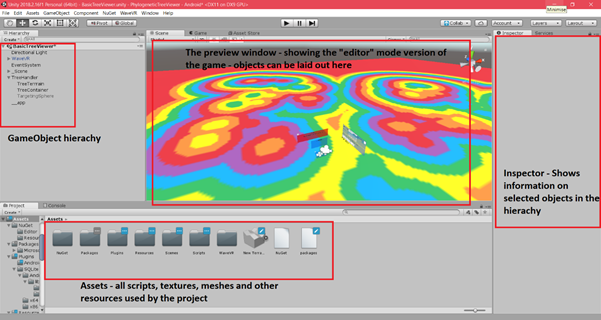
\includegraphics[width=\textwidth] {figures/UnityUI.png}}
\caption{{\bf The Unity UI.} Key areas are highlighted.}
\label{fig1}
\end{figure}

\subsection * {Algorithmic Components}
To achieve a feature rich visualisation system several core algorithms were developed; these will be explained in turn in this subsection.

\subsubsection * {Newick Parser} 
The first aspect of the project to be considered was the development of a parser capable of reading in Newick files and producing a coded representation of the contained tree. Fundamentally this algorithm broke down into two stages, tokenization and parsing. The tokenizer sub-algorithm was responsible for taking the input text file as a string and converting it into a sequence of valid tokens or rejecting the input as being lexically incorrect. The parser would then take the sequence of tokens and convert it into a final tree, or reject it as being syntactically incorrect. 

The tokenizer’s implementation was fairly straightforward as all tokens are single character length – the algorithm simply compares the head of the input text with the available tokens and saves the correct token to the output list. In the event that a character that is not recognised as a token is read, the algorithm can simply assume that a word is being read – this will either be an edge weight or a node label, and the result is a word token that can be written to the output list in the same way as all other token. For these reasons the Tokenise algorithm will run on any input string without the need to generate any errors; all error handling can be performed in the parsing algorithm instead.

The algorithm’s pseudocode implementation is as follows: 

\begin{algorithm}[H]
\SetAlgoLined
\SetKwData{ValidTokens}{valid\_tokens}\SetKwData{Tokens}{tokens}\SetKwData{Word}{word}
\SetKwData{ReadingWordFlag}{reading\_word\_flag} \SetKwData{Target}{target}
\SetKwInOut{Input}{input}\SetKwInOut{Output}{output}

\Input{A string \Target containing a newick descriptor}
\Output{A list of tokens \Tokens represented as strings}

\BlankLine

\ValidTokens$\leftarrow$ list of valid newick symbols\;
\Tokens$\leftarrow$ empty list of strings\;
\Word$\leftarrow$ ""\;
\ReadingWordFlag$\leftarrow$ false\;
\ForEach{character $c$ in \Target}{
	\eIf{\ValidTokens contains $c$}{
		\If{\ReadingWordFlag}{
			append \Word to \Tokens\;
			\ReadingWordFlag $\leftarrow$ false\;
		}
		append $c$ to \Tokens as a string\;
	}{
		\If {not \ReadingWordFlag}{
			\ReadingWordFlag $\leftarrow$ true\;
			\Word $\leftarrow$ ""\;
		}
		append $c$ to \Word\;
	}
}
\caption{Tokenizer}
\end{algorithm}

The list of tokens created by the tokenizer can be directly handed to the parser for parsing and generation of a final tree representation.  The parser loops through the generated tokens and, depending on the selected character, takes several actions culminating in the generation of a full tree structure in memory as one “Tree” object. Because of the deeply nested nature of trees and their Newick representations, the parser relies on the usage of a “node stack” that stores freshly created nodes; nodes are then popped from this stack and named in reverse order, depth first (from leaf nodes back to the root node). 

The algorithm’s pseudocode implementation is provided below as a helper function and a main algorithm:

%I tried breaking it into two algorithms so it would typeset across multiple pages but that didn't quite work :/ 
\begin{algorithm}[H]
\SetKwData{Tokens}{tokens}\SetKwData{CreatedTree}{created\_tree}
\SetKwData{Tree}{tree}\SetKwData{Name}{name}\SetKwData{NodeStack}{node\_stack}\SetKwData{Depth}{depth}
\SetKwData{TopNode}{top\_node} \SetKwData{ParentNode}{parent\_node}
\SetKwData{CreatedTree}{created\_tree} \SetKwData{ExpectNameFlag}{expect\_name\_flag} \SetKwData{LastNamedNode}{last\_named\_node}
\SetKwData{IsLabelFlag}{is\_label\_flag}
\SetKwData{Token}{token}

\SetKwInOut{Input}{input}\SetKwInOut{Output}{output}
\SetKwFunction{PopAndName}{popAndName}
\SetKwProg{Fn}{Function}{:}{}

\Input{A Tree object \Tree, a name label \Name, a node stack \NodeStack, a depth value \Depth}
\Output{A named node \TopNode from the node stack}

\BlankLine

\Fn {\PopAndName{\Tree, \Name, \NodeStack, \Depth}}{
	pop \TopNode from \NodeStack\;
	add \TopNode to \Tree\;
	\eIf{\Name == ""}{
		set \TopNode label to ""\;
	}{
		set \TopNode label to \Name\;
	}
	set \TopNode depth to \Depth\;
	\eIf {\NodeStack is not empty}{
		peek \ParentNode from \NodeStack\;
		\If{\ParentNode is not none}{
			add \TopNode as child of \ParentNode\;
			set \TopNode parent to \ParentNode\;
		}
	}{
		\If{\TopNode is not root of \Tree}{	
			SYNTAX\_ERROR\;
		}
	}
	return \TopNode\;
}
\caption{PopAndName function}
\end{algorithm}

%It won't go on one page or something I am not sure what to do here :'(
\begin{algorithm}[H]
\SetKwData{Tokens}{tokens}\SetKwData{CreatedTree}{created\_tree}
\SetKwData{Tree}{tree}\SetKwData{Name}{name}\SetKwData{NodeStack}{node\_stack}\SetKwData{Depth}{depth}
\SetKwData{TopNode}{top\_node} \SetKwData{ParentNode}{parent\_node}
\SetKwData{CreatedTree}{created\_tree} \SetKwData{ExpectNameFlag}{expect\_name\_flag} \SetKwData{LastNamedNode}{last\_named\_node}
\SetKwData{IsLabelFlag}{is\_label\_flag}
\SetKwData{Token}{token}

\SetKwInOut{Input}{input}\SetKwInOut{Output}{output}
\SetKwFunction{PopAndName}{popAndName}
\SetKwProg{Fn}{Function}{:}{}

\Input{A list of tokens \Tokens represented as strings}
\Output{A Tree object \CreatedTree}

\BlankLine

\CreatedTree $\leftarrow$ empty Tree\;
\NodeStack $\leftarrow$ empty Stack\;
\CreatedTree root $\leftarrow$ empty Node\;
push \CreatedTree root to \NodeStack\;
\Depth $\leftarrow$ 0\;

\BlankLine

\ExpectNameFlag $\leftarrow$ true\;
\LastNamedNode $\leftarrow$ none\;
\IsLabelFlag $\leftarrow$ false\;

\BlankLine

\ForEach{\Token in \Tokens}{
	\If{\Token length == 1}{
		\uIf{\Token first character == '('}{
			\Depth $\leftarrow$ \Depth + 1\;
			push new node to \NodeStack\;
			\ExpectNameFlag $\leftarrow$ true\;
		}
		\uElseIf{\Token first character == ')'}{
			\Depth $\leftarrow$ Depth - 1\;
			\If{\ExpectNameFlag}{
				\LastNamedNode $\leftarrow$ \PopAndName(\CreatedTree, none, \NodeStack, \Depth)\;
			}
			\ExpectNameFlag $\leftarrow$ false\;
		}
		\uElseIf{\Token first character == ','}{
			\If{\ExpectNameFlag}{
				\LastNamedNode $\leftarrow$ \PopAndName(\CreatedTree, none, \NodeStack, \Depth)\;
			}
			push new node to \NodeStack\;
			\ExpectNameFlag $\leftarrow$ true\;
		}
		\uElseIf{\Token first character == ';'}{
			\If{\ExpectNameFlag}{
				\LastNamedNode $\leftarrow$ \PopAndName(\CreatedTree, none, \NodeStack, \Depth)\;	
			}
		}
		\uElseIf{\Token first character == ''' or \Token first character == '"'}{
			continue
		}
		\uElseIf{\Token first character == ':'}{
			\If{\ExpectNameFlag}{
				\LastNamedNode $\leftarrow$ \PopAndName(\CreatedTree, none, \NodeStack, \Depth)\;	
			}
			\ExpectNameFlag $\leftarrow$ false\;
		}
		\uElse{
			\IsLabelFlag $\leftarrow$ true\;
		}
	}

	\BlankLine

	\If{\Token length > 1 or \IsLabelFlag}{
		\eIf{\ExpectNameFlag}{
			\LastNamedNode $\leftarrow$ \PopAndName(\CreatedTree, \Token, \NodeStack, \Depth)\;
			\ExpectNameFlag $\leftarrow$ false\;
		}{
			\eIf{\Token is edge weight}{
				\eIf{\LastNamedNode == none}{
					SYNTAX\_ERROR\;
				}{
					\LastNamedNode weight\_to\_parent $\leftarrow$
				}
			}{
				SYNTAX\_ERROR\;
			}
		}
	}
}
\BlankLine
\If{\NodeStack not empty}{
	SYNTAX\_ERROR\;
}
\caption{Parser}
\end{algorithm}

\subsubsection * {Two-Dimensional Tree Layout Algorithms}
Initially some work was put into into producing a two-dimensional layout algorithm for computing the initial tree layouts. This immediately highlighted the complexity of such algorithms. Generally, attempts at producing an efficient version of such an algorithm proved mostly futile, and with the high availability of graph visualisation/layout libraries already available it quickly became clear that this was attempting to “reinvent the wheel” by manually coding the basic layout algorithm. For this reason, it was decided to simplify the initial layout process with the addition of a graph visualisation algorithm – specifically the Microsoft Automatic Graph Layout library (MSAGL – discussed in more detail in the Methodology / Software Libraries section of this document). 

Ultimately to layout the tree in two dimensions my design became the following: parse a generic tree from a text file, adapt the tree to be MSAGL compliant, run MSAGL’s layout functions on that tree, then adapt the resulting MSAGL tree into Unity game objects to be rendered in 3D space.
Because of the high dependency on a rigidly implemented exterior library for layout, and its minimal nature, pseudo code will not be provided for this algorithm.

\subsubsection * {Three-Dimensional Tree Layout Algorithms}
To make basic use of the third dimension made available by the VR medium I designed a simple 3D transformation algorithm that takes a tree displayed in two dimensions and performs rotations along the axis of each branch to rotate the tree out of the plane. The algorithm takes as input a tree that is laid out on a plane using the “circular” view, then performs transformations upon it. This algorithm is quite straight forward in its implementation, the key concepts are shown in the following pseudocode implementation: 

%magical psuedocode formatting goes here
\begin{algorithm}[H]
\SetKwData{TargetTree}{target\_tree} \SetKwData{DegreesPerChild}{degrees\_per\_child}
\SetKwData{CurrentNode}{current\_node} \SetKwData{ChildNode}{child\_node}
\SetKwData{RotationAxis}{rotation\_axis} \SetKwData{RootNode}{root\_node}

\SetKwInOut{Input}{input}\SetKwInOut{Output}{output}
\SetKwFunction{RecursiveConstantRotate}{recursiveConstantRotate}
\SetKwProg{Fn}{Function}{:}{}

\Input{A Tree object \TargetTree passed by reference}
\Output{None - \TargetTree is mutated as a side effect}

\BlankLine

\Fn {\RecursiveConstantRotate{\CurrentNode}}{
	\DegreesPerChild $\leftarrow$ $n$ \tcc*[h]{0 < $n$ < 360}\;
	\ForEach{\ChildNode in \CurrentNode}{
		\RotationAxis $\leftarrow$ \ChildNode positon - \CurrentNode position\;
		rotate \ChildNode about \RotationAxis by \DegreesPerChild\;
		\RecursiveConstantRotate(\ChildNode)\;
	}
}

\BlankLine

\RecursiveConstantRotate(\RootNode from \TargetTree)\;
\caption{Recursive Rotation}
\end{algorithm}
	
The above algorithm recursively visits each node in the tree (if called from the root) and rotates it about the axis between itself and its parent by a fixed quantity. This has the beneficial effect of reducing the branch crossings that can sometimes be generated by the MSAGL library’s layout methods. It should be noted that the pseudo code assumes that the final implementation honours the hierarchical nature of the tree and applies any rotation to both the current node and its children.

\subsubsection * {Terrain Generation}
A key data view provided by this project is that of the terrain tree; this concept relies on utilising terrain height and shared terrain level to show node depth and node relationships respectively (see Fig~\ref{fig2} for an example of the final software implementation generating a tree). Generating the terrain took a considerable amount of computational effort and various versions of the generation algorithm. The process to create this algorithm will be explained in the following.

% This seems to just about go where ever it pleases
\begin{figure}[h!]
\center{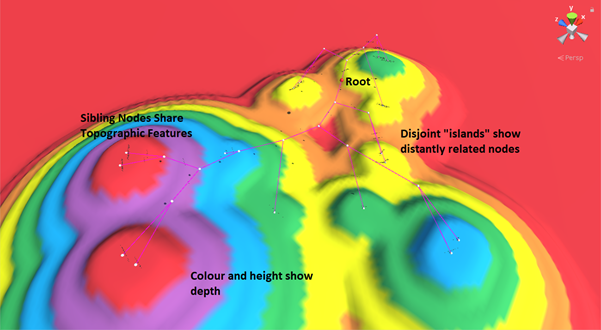
\includegraphics[width=\textwidth] {figures/TerrainExample.png}}
\caption{{\bf View of Terrain Tree.} Generated from a Newick file.}
\label{fig2}
\end{figure}

To facilitate terrain generation programmatically, Unity utilises a height map feature. That is to say that all terrain in Unity is essentially encoded by a two-dimensional array of floating-point height values, representing the height of a discrete section of terrain at a coordinate specified by the indices in the heightmap array. So, to edit a section of terrain at runtime one simply has to change the values stored within the heightmap array of the terrain.

The colour of the terrain is actually maintained in a similar way; each texture assigned to the terrain has an “alphamap” related to it, which dictates how strongly the texture is applied at any point within the terrain.

Initially the algorithm simply took the force directed two-dimensional layout from the MSAGL library, rotated it 90 degrees about the Z axis to sit on the plane, and elevated a circle at each node within the terrain to a height dependent upon the node’s depth. The result of this was unfortunately a terrain with little actual relevance to the tree data, and a generally poor representation of the tree itself.

This stage in development also highlighted the issue with nodes that were not siblings ending up too near each other in the final graph, resulting in terrains that spiked wildly in height from point to point, as a node of depth 10 might be a spatially close to a node of depth 6 for example. Similarly, it highlighted that iterating through the nodes in a depth first fashion, as we had, was a flawed decision.

Lastly during this step, it became clear that from a visual perspective some terrain smoothing would be necessary to make the generated features more visually pleasing.

To increase the information content of the generated terrain several steps were taken:

\begin{itemize}
	\item Node traversal in breadth first order
	\item Consider only leaf nodes when raising terrain
	\item Application of a custom written force directed algorithm to bring sibling leaf nodes closer together and to repel non-sibling leaf nodes
	\item Application of a smoothing algorithm to counter jagged edges in the terrain
\end{itemize}


The first major step in developing suitable terrain was the application of a static force directed algorithm to group related nodes and repel non-related nodes, a concept that was inferred from the work of Waese and company \cite{bib3}. While Waese et al’s algorithm for force directed layout is applied at run time continuously “until a stable configuration is reached” \cite{bib3}, the algorithm employed in this case has to run a fixed number of times before the terrain is raised, as editing the terrain is too computationally expensive to be done at run time in the same way (due to the way in which heightmaps are stored and edited within Unity).

The developed algorithm therefore considers each leaf node in turn, then applies an attraction force to it and all sibling nodes that is equal to a force vector \textit{Fbase} multiplied by the square of the distance between the two nodes dist. This means that at large ($dist > 1$) distances the two nodes are attracted together by a large force, while at smaller distances ($dist < 1$) the attraction force rapidly decreases. For every non-sibling node an opposite operation is performed: the two nodes are repelled from each other by \textit{-Fbase} divided by the distance squared; this means that at small distances the repulsion force will be very large but will quickly diminish at greater distances.

The algorithm’s pseudocode implementation is shown below: 

%pretty psuedocode formatting
\begin{algorithm}[H]
\SetKwData{LeafNodes}{leaf\_nodes} \SetKwData{CurrentNode}{current\_node} \SetKwData{OtherNode}{other\_nodes}
\SetKwData{DistSquared}{dist\_squared}

\SetKwInOut{Input}{input}\SetKwInOut{Output}{output}

\Input{A list of leaf nodes \LeafNodes from a Tree object passed by reference}
\Output{None - nodes are mutated as a side effect}

\ForEach{\CurrentNode in \LeafNodes}{
	\ForEach{\OtherNode in \LeafNodes}{
		\DistSquared $\leftarrow$ square of distance from \CurrentNode to \OtherNode\;
		\eIf{\CurrentNode and \OtherNode are siblings}{
			\If{\DistSquared $>$ min distance}{
				move \CurrentNode and \OtherNode toward each other\;
			}
		}{
			move \CurrentNode and \OtherNode away from each other\;
		}
	}
}
\caption{Pass}
\end{algorithm}

The above algorithm is applied to the list of leaf nodes 40 times at tree generation time, resulting in tightly grouped sibling nodes and clear spatial separation between all other leaf nodes.


Smoothing a terrain heightmap is essentially an image processing problem, so to achieve my aims I implemented a simple mean box filter that uses averages to reduce harsh edges in the terrain. The algorithm essentially replaces the value of each heightmap point with the average value of its neighbours within a specified area. This algorithm is then applied a number of times in discrete passes to generate the final smoothed terrain. Ultimately it became clear that over smoothing the terrain had two problems – firstly having clear divisions between height levels was useful for data representation, and secondly that a high degree of smoothing was very computationally expensive to obtain. For this reason, I opted to utilise only a small number of passes and to average each point only with its immediate neighbours. The result of this smoothing can be seen again in figure 6.
The pseudocode implementation for the inner smooth function “SmoothPass” is shown below:

\begin{algorithm}[H]

\SetKwData{Heights}{heights} \SetKwData{SmoothRadius}{smooth\_radius}
\SetKwData{NewHeights}{new\_heights}
\SetKwData{HeightMapWidth}{height\_map\_width} \SetKwData{HeightMapHeight}{height\_map\_height}
\SetKwData{Column}{column} \SetKwData{Row}{row}
\SetKwData{Count}{count} \SetKwData{Total}{total} \SetKwData{Value}{value}

\SetKwInOut{Input}{input}\SetKwInOut{Output}{output}

\Input{A 2D list (matrix) of heights (numbers) \Heights, a radius \SmoothRadius}
\Output{A 2D list (matrix) of heights (numbers) \NewHeights}

\BlankLine

\HeightMapWidth $\leftarrow$ $x$ dimension of \Heights\;
\HeightMapHeight $\leftarrow$ $y$ dimension of \Heights\;
\NewHeights $\leftarrow$ copy of \Heights\;

\BlankLine

\ForEach{\Column in \Heights}{ 
	\ForEach{\Row in \Heights}{
		\Count $\leftarrow$ 0\;
		\Total $\leftarrow$ 0\;
		\ForEach{\Value in \Heights within \SmoothRadius}{
			\Count $\leftarrow$ \Count + 1\;
			\Total $\leftarrow$ \Total + \Value\;
		}
		\NewHeights at \Row, \Column $\leftarrow$ \Total / \Count\;
	}
}
\caption{Smooth Pass}
\end{algorithm}

At this point the terrain was both smooth and well grouped, but each node still appeared to sit on a “pillar” of terrain rather than in a fully layered topographic “landscape” as was the aim. To produce a more meaningful terrain two alterations to the generation process were required. Firstly, the terrain raising process was changed so that each node raised a set of concentric circles of increasing height and decreasing diameter – resulting in a “stack” of terrain appearing naturally beneath each node. Secondly, the method in which changes to the terrain occurred was altered by ensuring that an area of terrain’s height would only be changed if the new height represented an increase to the terrain’s height at that point. This ensured that the terrain would not be overridden or “clipped” by a disk of lower level being created in the same area as another disk of higher level (see Fig~\ref{fig3}).

% This seems to just about go where ever it pleases
\begin{figure}[h!]
\center{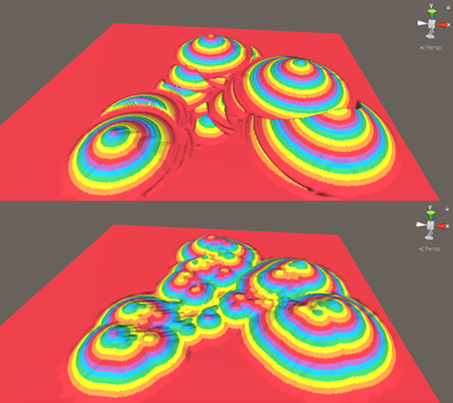
\includegraphics {figures/TerrainClipping.png}}
\caption{{\bf Height Clipping.} Height overriding created by the lower disks of terrain generated for deeper nodes in the tree (top), vs the true terrain generated with a height comparison before assignment.}
\label{fig3}
\end{figure}

The pseudocode implementation of the final terrain raising algorithm is shown below:

%pretty psuedocode formatting 
\begin{algorithm}[H]
\SetKwData{BFSOrderedLeafNodes}{BFS\_ordered\_leaf\_nodes} \SetKwData{CurrentNode}{current\_node}
\SetKwData{HeightIncrement}{height\_increment} \SetKwData{CurrentDepth}{current\_depth}
\SetKwData{MinSize}{min\_size} \SetKwData{Size}{size} \SetKwData{Heights}{heights}
\SetKwData{RadiusSquared}{radius\_squared} \SetKwData{Center}{center} \SetKwData{DistSquared}{dist\_squared}
\SetKwData{IndexPos}{index\_pos} \SetKwData{Val}{val}

\SetKwInOut{Input}{input}\SetKwInOut{Output}{output}

\Input{A list of leaf nodes \BFSOrderedLeafNodes constructed breadth first}
\Output{None - mutates heights contained within terrain as a side effect}

\BlankLine
\tcc*[h]{$<$x, y$>$ indicates a vector with components x and y}\;
\ForEach{\CurrentNode in \BFSOrderedLeafNodes}{
	\HeightIncrement $\leftarrow$ 0.01\; 
	\CurrentDepth $\leftarrow$ 0\;
	\MinSize $\leftarrow$ 20\;
	\While {\CurrentDepth $<$ \CurrentNode depth}{
		\Size $\leftarrow$ (\CurrentNode depth - \CurrentDepth + 1) * \MinSize\;
		\Heights $\leftarrow$ terrain height map around \CurrentNode\;
		\RadiusSquared $\leftarrow$ (\Size * \Size) / 4\;
		\Center $\leftarrow$ $<$ \Size / 2, \Size / 2] $>$ \;
		\For{$i$ in range 0 to \Size}{	
			\For{$j$ in range 0 to \Size}{		
				\IndexPos $\leftarrow$ $<$ $i$, $j$ $>$ \;
				\DistSquared $\leftarrow$ square of distance between \IndexPos and \Center
				\If{\DistSquared $<$ \RadiusSquared}{
					\Val $\leftarrow$ \HeightIncrement * \CurrentDepth\;
					\If{\Val $>$ \Heights[$i$, $j$]}{
						\Heights[$i$, $j$] $\leftarrow$ \Val\;
					}
				}
			}
		}
		update terrain heightmap at \CurrentNode with \Heights\;	
		\CurrentDepth $\leftarrow$ \CurrentDepth + 1\;
	}
}

\caption{Terrain Raising}

\end{algorithm}

Ultimately the above functions are combined in a specific order to produce the final terrain, along with the addition of caching functionality to write terrain heights to a text file – to reduce the time and computational requirement of generating larger trees. The final high-level pseudo terrain generation function is as follows: 


%psuedocode formatting
\begin{algorithm}[H]
\SetKwData{OnFrameLoadingFlag}{on\_frame\_loading\_flag} \SetKwData{NumRaisesPerFrame}{num\_raises\_per\_frame}
\SetKwData{CurrentBuildStep}{current\_build\_step} \SetKwData{ForceDirectedLayout}{force\_directed\_layout}
\SetKwData{CheckForCachedHeights}{check\_for\_cached\_heights} \SetKwData{NodeRaising}{node\_raising}
\SetKwData{TerrainRaising}{terrain\_raising} \SetKwData{BFSQueueNodes}{bfs\_queue\_nodes}
\SetKwData{CurrentNode}{current\_node} \SetKwData{TerrainSmoothing}{terrain\_smoothing}
\SetKwData{TerrainColouring}{terrain\_colouring} \SetKwData{NewHeights}{new\_heights}

\SetKwInOut{Input}{input}\SetKwInOut{Output}{output}

\SetKwBlock{OncePerFrame}{$once\_per\_frame$ begin}{end}

\Input{None - runs on frame update if \OnFrameLoadingFlag is true}
\Output{None - mutates state of world objects as a side effect}

\BlankLine

\NumRaisesPerFrame $\leftarrow$ 10\;
\CurrentBuildStep $\leftarrow$ \ForceDirectedLayout\;

\BlankLine
\OncePerFrame{
	\If{\OnFrameLoadingFlag}{
		\uIf{\CurrentBuildStep == \ForceDirectedLayout}{
			perform force pass on leaf nodes of tree\;
			\If{number of passes performed $>=$ number required}{
				\CurrentBuildStep $\leftarrow$ \CheckForCachedHeights\;
			}
		}
		\uElseIf{\CurrentBuildStep == \CheckForCachedHeights}{
			\eIf{heights exist}{	
				load heights from cache\;
				\CurrentBuildStep $\leftarrow$ \NodeRaising\;
			}{
				\CurrentBuildStep $\leftarrow$ \TerrainRaising\;
			}
		}
		\uElseIf{\CurrentBuildStep == \TerrainRaising}{
			\If{\BFSQueueNodes is none}{
				\BFSQueueNodes $\leftarrow$ new queue\;
				enqueue $root$ into \BFSQueueNodes\;
			}
			\For{$i$ in range 0 to \NumRaisesPerFrame}{
				\eIf{\BFSQueueNodes is not empty}{
					dequeue \CurrentNode from \BFSQueueNodes\;
					\eIf{\CurrentNode is leaf}{
						raise terrain to \CurrentNode \;
					}{
						enqueue all children of \CurrentNode to \BFSQueueNodes\;
					}
				}{
					\CurrentBuildStep $\leftarrow$ \TerrainSmoothing\;	
					$break$\;
				}
			}
		}
		\uElseIf{\CurrentBuildStep == \TerrainSmoothing}{
			smooth terrain \;
			cache terrain heights\;
			\CurrentBuildStep $\leftarrow$ \NodeRaising\;
		}
		\uElseIf{\CurrentBuildStep == \NodeRaising}{
			raise nodes above terrain\;
			raise user above terrain\;
			\CurrentBuildStep $\leftarrow$ \TerrainColouring\;
		}
		\uElseIf{\CurrentBuildStep == \TerrainColouring}{
			colour terrain based on \NewHeights\;
			\OnFrameLoadingFlag $\leftarrow$ false\;
			\CurrentBuildStep $\leftarrow$ \ForceDirectedLayout\;
		}
	}
}
\caption{On Frame Loading}
\end{algorithm}

The function is designed to be run once per frame, each time completing a step or sub step in the full terrain generation process. This is done to ensure that the software doesn’t become completely unresponsive during terrain building.

\subsubsection {Metainformation and SQLite databases}

An important element of this project was developing a sensible method of storing and retreiving meta information. Initially it had been suggested to perhaps support a different tree file standard with built in constructs for this data, but as the Newick format is so pervasive in current literature it made more sense to offer support for SQLite databases containing information on nodes.
 
To enable correct support for SQLite was unfortunately a non-trivial issue; Android has native support for SQLite databases (this is ultimately the target build platform for the project), but Unity unfortunately offers no such support. Therefore, to enable the utilization of databases a plugin developed under the MIT permissive license was used, developed by Asif R and made available through GitHub. The article explaining this plugin’s use and linking to the GitHub repository is available via \cite{bib6}. With this plugin included in the Unity build a script DBQueries could be written to facilitate the querying of a database. 
The aim of this inclusion was to allow the user to provide a separate database file with the same name as a given tree but the “.db” file extension. This is then loaded by my software and checked for a “metainformation” table; the table is expected to be indexed by a primary key column labelled “id”. If the table matches the expected format column names are extracted and stored, and then using standard SQLite queries (via Asif R’s SQLite plugin 2018 \cite{bib6}) the table is queried for information with relation to each node in the tree using a simple SELECT/FROM command filtered by ID. Each node’s internal string variable “metainformation” is then updated to be a concatenation of all displayable data from the tree tagged with its column name. 

Additional unity scripts are then used at run time to display the metainformation to the user when they hover over a node. An example meta information panel is shown in Fig~\ref{fig4}

% This seems to just about go where ever it pleases
\begin{figure}[h!]
\center{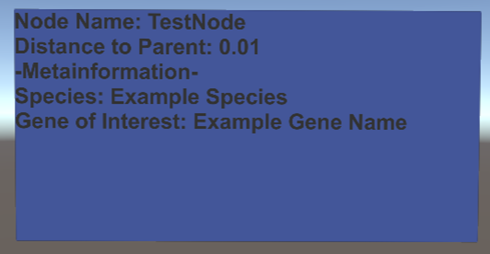
\includegraphics[width=\textwidth] {figures/MetaExample.png}}
\caption{{\bf Example metainformation panel.} Generated from associated SQLite database.}
\label{fig4}
\end{figure}


% Results and Discussion can be combined.
\section*{Results}

The developed software is capable of representing small to medium / large sized trees efficiently, with a high degree of accuracy in terms of the terrain layouts generated. It takes around a minute to fully generate the terrain for larger trees, but this is then cached to the device storage so that the computation doesn't have to be repeated. The other views provided all generate rapidly, and there is discernable lag from the user's perspective. 

By utilising each of the data views provided, a user can easily glean key information about a tree of interest. The user can load the tree in the terrain view to understand high level information, then "zoom in" or switch to one of the other more basic tree views to understand specific areas of interest. This is a unique way of understanding tree data that - to the author's knowledge - has not as yet been replicated. There is a high degree of potential for both this software and any others that are capable of representing trees in a multitude of ways to maximise the efficiency with which researchers can understand them. 

\section*{Discussion}

The software developed for this project proved to be a novel and unique first step into the possibilities of representing phylogenetic information in VR. Both the algorithms and the final application serve as an excellent indicator of the potential of using VR for viewing phylogenetic data along with applying to the area of data visualisation as a whole. The data views developed provide an excellent accompaniment to the standard tree diagram - by both extending it with supplementary meta information, and by altering it altogether and displaying it as a terrain based view. 

From the current state of the project there are a great number of potential improvements and additions one could make to the software. While in conversation with an end user a good number of these suggestions were brought up. Namely it became apparent that while this project represented a good start in the realm of displaying phylogenetic trees, there was a great deal of potential for other information visualisation methods to be developed. 

Firstly, in terms of concrete improvements, the terrain view implemented would benefit greatly from including a better representation of phylogenetic distance (as suggested during user testing). The terrain layout algorithm could be altered to achieve this without too much difficulty, although it would be necessary to manufacture the algorithm to ensure that the application does not become unresponsive. 

Secondly, a more consistent and clear way of managing tree files would be helpful; perhaps the inclusion of an online service to transfer files to the device could be of use, allowing the user to simply upload their newick files to a website and then access them through the app “on device”. This could also perhaps apply to tree terrain generation also – the terrain could be generated using a cloud computing service and the resulting heightmap passed cached on to the device instead, reducing the amount of computation that need be done on the comparatively slow headset processor.

Thirdly, it could be prudent to put some time into researching ways of allowing users to see both high- and low-level features of trees – and to give them fluid methods of transitioning between these views. Perhaps this could take the form of a terrain that represented the high-level features and spacing of nodes, with the view transitioning into a clearer branching local structure as the user zoomed in? There is a great deal of potential in this area, and a full design team working in contact with actual researchers in the field could make great strides in improving the usability and usefulness of VR visualisation systems.
Fourthly, there is an opening for a system that is able to show the different possible trees that can be created from the same species; given a group of species one can construct an evolutionary tree between them based on the inheritance of one gene that might be wildly different from another tree generated based on the inheritance of a separate gene. A system that could show the variations in these trees and highlight how the models vary based on the supplied information could be a fantastic tool for researchers.

Fifth, the importance of efficiency must be considered. As pointed out previously there is a vast amount of data available, and any tool capable of representing modern trees with their potentially thousands if not millions of leaf nodes is likely to be invaluable to researchers. 

Ultimately through working on this project it has become clear that new and better visualisation tools are needed, and in whatever medium they take they have to meet one key requirement: They must be “better than just using a bigger piece of paper” (as pointed out by Dr K. Winzer during testing). Whatever systems are developed must represent an actual benefit for the target audience vs simply printing a cladogram out and annotating it by hand – there has to be a proper translation from the academic task of designing the systems to the actual implementation and usefulness of said systems. The system we developed proves that visualising phylogenetic trees in VR is both possible and an area worthy of further study but ultimately could be extended and improved immensely with more time and more developers. 

\section*{Acknowledgments}
We extend thanks to Dr K. Winzer for discussing the final application with us and giving useful feedback on potential future improvements.

\nolinenumbers

\begin{thebibliography}{10}

\bibitem{bib1}
Emery L.
\newblock Why is pylogenetics important?
\newblock \textit{European Bioinformatics Institute [Internet]}. 
\newblock 2014 May [cited 2018 May 05];9(12):[about 1p.].
\newblock Available from: \href{https://www.ebi.ac.uk/training/online/course/introduction-phylogenetics/why-phylogenetics-important}{https://www.ebi.ac.uk/training/online/course/introduction-phylogenetics/why-phylogenetics-important}

\bibitem{bib2}
Carrizo SF.
\newblock Phylogenetic Trees: An Information Visualisation Perspective.
\newblock \textit{Proceedings of the Second Conference on Asia-Pacific Bioinformatics - Volume 29}. 
\newblock 2004 Jan; 29: 315–320 
\newblock Available from: \href{https://dl.acm.org/citation.cfm?id=976520.976563}{https://dl.acm.org/citation.cfm?id=976520.976563} [Accessed 2019 June 16]

\bibitem{bib3}
Waese J, Provart NJ, Guttman DS.
\newblock Topo-phylogeny: Visualizing evolutionary relationships on a topographic landscape.
\newblock \textit{PLoS ONE}.
\newblock 2017 May; 12(5): e0175895. Available from: \href{https://doi.org/10.1371/journal.pone.0175895}{https://doi.org/10.1371/journal.pone.0175895}

\bibitem{bib4}
Forghani M, Vasev P, Averbukh V.
\newblock A Visualization System for Binary Rooted Trees.
\newblock \textit{Scientific Visualisation}. 
\newblock 2017 Dec; 9(4):59-66. Available from: \href{http://sv-journal.org/2017-4/06/index.php?lang=en}{http://sv-journal.org/2017-4/06/index.php?lang=en}
\newblock doi: 10.26583/sv.9.4.06.

\bibitem{bib5}
Craighead J, Burke J, Murphy R.
\newblock Using the unity game engine to develop sarge: a case study.
\newblock \textit{Computer}
\newblock 2007 Jan [cited 2019 Jun 18]; 4552. 
\newblock Available from: \href{https://www.researchgate.net/publication/265284198\_Using\_the\_Unity\_Game\_Engine\_to\_Develop\_SARGE\_A\_Case\_Study}{https://www.researchgate.net/publication/265284198\_Using\_the\_Unity\_Game\_Engine\_to\_Develop\_SARGE\_A\_Case\_Study}

\bibitem{bib6}
Asif R 
\newblock \textit{SQLite and unity: how to do it right.}
\newblock Available from: \href{https://medium.com/@rizasif92/sqlite-and-unity-how-to-do-it-right-31991712190}{https://medium.com/@rizasif92/sqlite-and-unity-how-to-do-it-right-31991712190}
\newblock [Accessed 2019 Jun 20]

\end{thebibliography}

\end{document}

